\documentclass{standalone}
\usepackage{tikz}
\usepackage{ctex,siunitx}
\setCJKmainfont{Noto Serif CJK SC}
\usepackage{tkz-euclide}
\usepackage{amsmath}
\usetikzlibrary{patterns, calc,3d}
\usetikzlibrary {decorations.pathmorphing,decorations.pathreplacing,decorations.shapes}
\tikzset{label style/.append style={font=\small}}
\begin{document}
\small
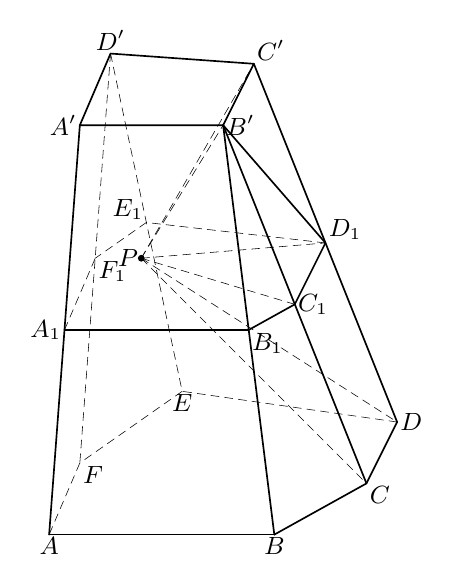
\begin{tikzpicture}[>=latex,scale=1.3,inner sep=1pt]
  \tkzDefPoints{0/0/A,2.2/0/B,3.1/0.5/C,3.4/1.1/D,1.3/1.4/E,0.3/0.7/F}
  \tkzDefPoints{0.3/4/A',1.7/4/B',0.9/2.7/P}
  \tkzDefPointsBy[translation=from A to A'](F){D'}
  \tkzDefPointsBy[translation=from C to B'](D){C'}
  \tkzDefMidPoint(A,A')\tkzGetPoint{A1}
  \tkzDefMidPoint(B,B')\tkzGetPoint{B1}
  \tkzDefMidPoint(C,B')\tkzGetPoint{C1}
  \tkzDefMidPoint(C',D)\tkzGetPoint{D1}
  \tkzDefMidPoint(E,D')\tkzGetPoint{E1}
  \tkzDefMidPoint(F,D')\tkzGetPoint{F1}
  \tkzDrawPoints[fill=black](P)

  \tkzDrawSegments[semithick](A,B B,C C,D A',A B',B B',C C',D A1,B1 B1,C1 C1,D1 B',D1)
  \tkzDrawSegments[densely dashed](E,F F,A D',F D',E D,E A1,F1 D1,E1 E1,F1 P,C' P,B' P,D1 P,C1 P,C P,D)
  \tkzDrawPolygon[semithick](A',B',C',D')
  \tkzLabelPoints(A,B,E)
  \tkzLabelPoints[below right](C,F)
  \tkzLabelPoints[right](D,B')
  \tkzLabelPoints[left](A',P)
  \tkzLabelPoints[above](D')
  \tkzLabelPoints[above right](C')
  \tkzLabelPoint[left](A1){$A_1$}
  \tkzLabelPoint[below right](B1){$B_1$}
  \tkzLabelPoint[right](C1){$C_1$}
  \tkzLabelPoint[above right](D1){$D_1$}
  \tkzLabelPoint[above left](E1){$E_1$}
  \tkzLabelPoint[below right](F1){$F_1$}
\end{tikzpicture}
\end{document}